
\documentclass[ review  , 3p ]{elsarticle}
%default = preprint (single sapce), review = doublespace
%detail class option: https://www.elsevier.com/__data/assets/pdf_file/0008/56843/elsdoc-1.pdf

% eliminate "Preprinted to Elsevier"
\makeatletter
\def\ps@pprintTitle{%
 \let\@oddhead\@empty
 \let\@evenhead\@empty
 \def\@oddfoot{\centerline{\thepage}}%
 \let\@evenfoot\@oddfoot}
\makeatother

%%% Begin My package additions %%%%%%%%%%%%%%%%%%%
\usepackage[hyphens]{url}



\usepackage{lineno} % add
\providecommand{\tightlist}{%
  \setlength{\itemsep}{0pt}\setlength{\parskip}{0pt}}

\usepackage{graphicx}

\usepackage{zxjatype}
\usepackage{xeCJK}
\setCJKmainfont{ipaexm.ttf}
\setCJKsansfont{ipaexg.ttf}
\setCJKmonofont{ipaexg.ttf}

\usepackage{color}

\usepackage{booktabs}
\usepackage{longtable}
\usepackage{array}
\usepackage{multirow}
\usepackage{wrapfig}
\usepackage{float}
\usepackage{colortbl}
\usepackage{pdflscape}
\usepackage{tabu}
\usepackage{threeparttable}
\usepackage{threeparttablex}
\usepackage[normalem]{ulem}
\usepackage{makecell}
\usepackage{xcolor}


%\usepackage{xpatch}
%\xpatchcmd{\MaketitleBox}{\hrule}{}{}{}% remove first horizontal rule (above abstract)
%\xpatchcmd{\MaketitleBox}{\hrule}{}{}{}% remoce second horizonral rule (below keywords)
%%%%%%%%%%%%%%%% end my additions to header

\usepackage[T1]{fontenc}
\usepackage{lmodern}
\usepackage{amssymb,amsmath}
\usepackage{ifxetex,ifluatex}
\usepackage{fixltx2e} % provides \textsubscript
% use upquote if available, for straight quotes in verbatim environments
\IfFileExists{upquote.sty}{\usepackage{upquote}}{}
\ifnum 0\ifxetex 1\fi\ifluatex 1\fi=0 % if pdftex
  \usepackage[utf8]{inputenc}
\else % if luatex or xelatex
  \usepackage{fontspec}
  \ifxetex
    \usepackage{xltxtra,xunicode}
  \fi
  \defaultfontfeatures{Mapping=tex-text,Scale=MatchLowercase}
  \newcommand{\euro}{€}
\fi
% use microtype if available
\IfFileExists{microtype.sty}{\usepackage{microtype}}{}
\bibliographystyle{elsarticle-harvard}
\usepackage{tabularx}
\ifxetex
  \usepackage[setpagesize=false, % page size defined by xetex
              unicode=false, % unicode breaks when used with xetex
              xetex]{hyperref}
\else
  \usepackage[unicode=true]{hyperref}
\fi
\hypersetup{breaklinks=true,
            bookmarks=true,
            pdfauthor={},
            pdftitle={Short Paper},
            colorlinks=false,
            urlcolor=blue,
            linkcolor=magenta,
            pdfborder={0 0 0}}
\urlstyle{same}  % don't use monospace font for urls

\setcounter{secnumdepth}{5}

\newlength{\cslhangindent}
\setlength{\cslhangindent}{1.5em}
\newlength{\csllabelwidth}
\setlength{\csllabelwidth}{3em}
\newenvironment{CSLReferences}[3] % #1 hanging-ident, #2 entry spacing
 {% don't indent paragraphs
  \setlength{\parindent}{0pt}
  % turn on hanging indent if param 1 is 1
  \ifodd #1 \everypar{\setlength{\hangindent}{\cslhangindent}}\ignorespaces\fi
  % set entry spacing
  \ifnum #2 > 0
  \setlength{\parskip}{#2\baselineskip}
  \fi
 }%
 {}
\usepackage{calc} % for \widthof, \maxof
\newcommand{\CSLBlock}[1]{#1\hfill\break}
\newcommand{\CSLLeftMargin}[1]{\parbox[t]{\maxof{\widthof{#1}}{\csllabelwidth}}{#1}}
\newcommand{\CSLRightInline}[1]{\parbox[t]{\linewidth}{#1}}
\newcommand{\CSLIndent}[1]{\hspace{\cslhangindent}#1}

% Pandoc toggle for numbering sections (defaults to be off)


% Pandoc header


\begin{document}
  \begin{frontmatter}

    \title{Charitable Giving, Tax Reform, and Government Efficiency\tnoteref{1}}
            \tnotetext[1]{This research is base on}
                \author[Osaka University]{
      Hiroki Kato 
       \corref{*} }
     \ead{vge008kh@stundent.econ.osaka-u.ac.jp}   %to avoid auto-link, use \@ instead of @
        \author[Chiba University]{
      Tsuyoshi Goto 
      }
      %to avoid auto-link, use \@ instead of @
        \author[Kobe University]{
      Yong-Rok Kim 
      }
      %to avoid auto-link, use \@ instead of @
            \address[Osaka University]{Graduate School of Economics, Osaka University, Japan}
        \address[Chiba University]{Graduate School of Economics, Chiba University, Japan}
        \address[Kobe University]{Graduate School of Economics, Kobe University, Japan}
            \cortext[*]{Corresponding Author.}
      
        \begin{abstract}
      Brah
    \end{abstract}
      
        \begin{keyword}
      Charitable giving, Giving price, Tax reform, Governement efficiency, South Korea
       \JEL{D91, I10, I18} 
    \end{keyword}
    
  \end{frontmatter}

  \hypertarget{introduction}{%
  \section{Introduction}\label{introduction}}
  
  Placeholder
  
  \hypertarget{charitable-giving-and-taxiation}{%
  \subsection{Charitable Giving and Taxiation}\label{charitable-giving-and-taxiation}}
  
  \hypertarget{summary-in-short}{%
  \subsection{Summary in short}\label{summary-in-short}}
  
  \hypertarget{south-korean-tax-reform}{%
  \subsection{South Korean tax reform}\label{south-korean-tax-reform}}
  
  \hypertarget{related-literature}{%
  \subsection{Related Literature}\label{related-literature}}
  
  \hypertarget{research-about-tax-price-elasticity-of-charitable-donations}{%
  \subsection{Research about tax price elasticity of charitable donations}\label{research-about-tax-price-elasticity-of-charitable-donations}}
  
  \hypertarget{research-about-perception-towards-the-government-and-donationtax-payment.}{%
  \subsection{Research about perception towards the government and donation/tax payment.}\label{research-about-perception-towards-the-government-and-donationtax-payment.}}
  
  \hypertarget{why-political-trust}{%
  \subsection{Why Political Trust?}\label{why-political-trust}}
  
  \hypertarget{institutional-background}{%
  \section{Institutional background}\label{institutional-background}}
  
  Placeholder
  
  \hypertarget{tax-relief-for-charitable-giving-by-tax-deduction-and-tax-credit}{%
  \subsection{Tax relief for charitable giving by tax deduction and tax credit}\label{tax-relief-for-charitable-giving-by-tax-deduction-and-tax-credit}}
  
  \hypertarget{korean-tax-reform-in-2014-need-modification-by-kim-san}{%
  \subsection{Korean tax reform in 2014 (Need modification by Kim san)}\label{korean-tax-reform-in-2014-need-modification-by-kim-san}}
  
  \hypertarget{data}{%
  \section{Data}\label{data}}
  
  Placeholder
  
  \hypertarget{national-survey-of-tax-and-benefit-nastab}{%
  \subsection{National Survey of Tax and Benefit (NaSTaB)}\label{national-survey-of-tax-and-benefit-nastab}}
  
  \hypertarget{time-series-of-chariable-giving}{%
  \subsection{Time Series of Chariable Giving}\label{time-series-of-chariable-giving}}
  
  \hypertarget{summary-statistics}{%
  \subsection{Summary Statistics}\label{summary-statistics}}
  
  \hypertarget{what-is-giving-price}{%
  \subsection{What is Giving Price?}\label{what-is-giving-price}}
  
  \hypertarget{determination-of-tax-amount}{%
  \subsection{Determination of Tax Amount}\label{determination-of-tax-amount}}
  
  \hypertarget{derive-giving-price}{%
  \subsection{Derive Giving Price}\label{derive-giving-price}}
  
  \hypertarget{construct-giving-price}{%
  \subsection{Construct Giving Price}\label{construct-giving-price}}
  
  \hypertarget{income-distribution-and-giving-price}{%
  \subsection{Income Distribution and Giving Price}\label{income-distribution-and-giving-price}}
  
  \hypertarget{empirical-strategy}{%
  \subsection{Empirical Strategy}\label{empirical-strategy}}
  
  \hypertarget{intensive-margin-and-extensive-margin}{%
  \subsection{Intensive Margin and Extensive Margin}\label{intensive-margin-and-extensive-margin}}
  
  \hypertarget{main-results}{%
  \section{Main Results}\label{main-results}}
  
  Placeholder
  
  \hypertarget{price-and-income-elasticity}{%
  \subsection{Price and Income Elasticity}\label{price-and-income-elasticity}}
  
  \hypertarget{baseline-regressions-result}{%
  \subsection{Baseline Regressions: Result}\label{baseline-regressions-result}}
  
  \hypertarget{intensive-margin-and-extensive-margin-result}{%
  \subsection{Intensive Margin and Extensive Margin: Result}\label{intensive-margin-and-extensive-margin-result}}
  
  \hypertarget{robustness-check}{%
  \subsection{Robustness Check}\label{robustness-check}}
  
  \hypertarget{robustness-check-1}{%
  \subsection{Robustness Check 1}\label{robustness-check-1}}
  
  \hypertarget{robustness-check-1-result}{%
  \subsection{Robustness Check 1: Result}\label{robustness-check-1-result}}
  
  \hypertarget{robustness-check-1-intensive-and-extensive-margin}{%
  \subsection{Robustness Check 1: Intensive and Extensive Margin}\label{robustness-check-1-intensive-and-extensive-margin}}
  
  \hypertarget{robust-check-2}{%
  \subsection{Robust Check 2}\label{robust-check-2}}
  
  \hypertarget{robustness-check-2-result}{%
  \subsection{Robustness Check 2: Result}\label{robustness-check-2-result}}
  
  \hypertarget{robustness-check-2-intensive-and-extensive-margin}{%
  \subsection{Robustness Check 2: Intensive and Extensive Margin}\label{robustness-check-2-intensive-and-extensive-margin}}
  
  \hypertarget{governement-efficient-and-price-elasticity}{%
  \section{Governement Efficient and Price Elasticity}\label{governement-efficient-and-price-elasticity}}
  
  \hypertarget{government-efficiency}{%
  \subsection{Government Efficiency}\label{government-efficiency}}
  
  From the 2015 survey,
  NaSTaB asks the current and ideal balance between tax burden and welfare size.
  
  These variables provide us to investigate the relationship between price elasticity and govenrment's efficiency
  more directly.
  
  Thus, we did same excercise, using the current balance bewteen tax burden and welfare size.
  
  \hypertarget{construct-efficient-index}{%
  \subsection{Construct Efficient Index}\label{construct-efficient-index}}
  
  Questionnaire of tax-welfare balance index is
  
  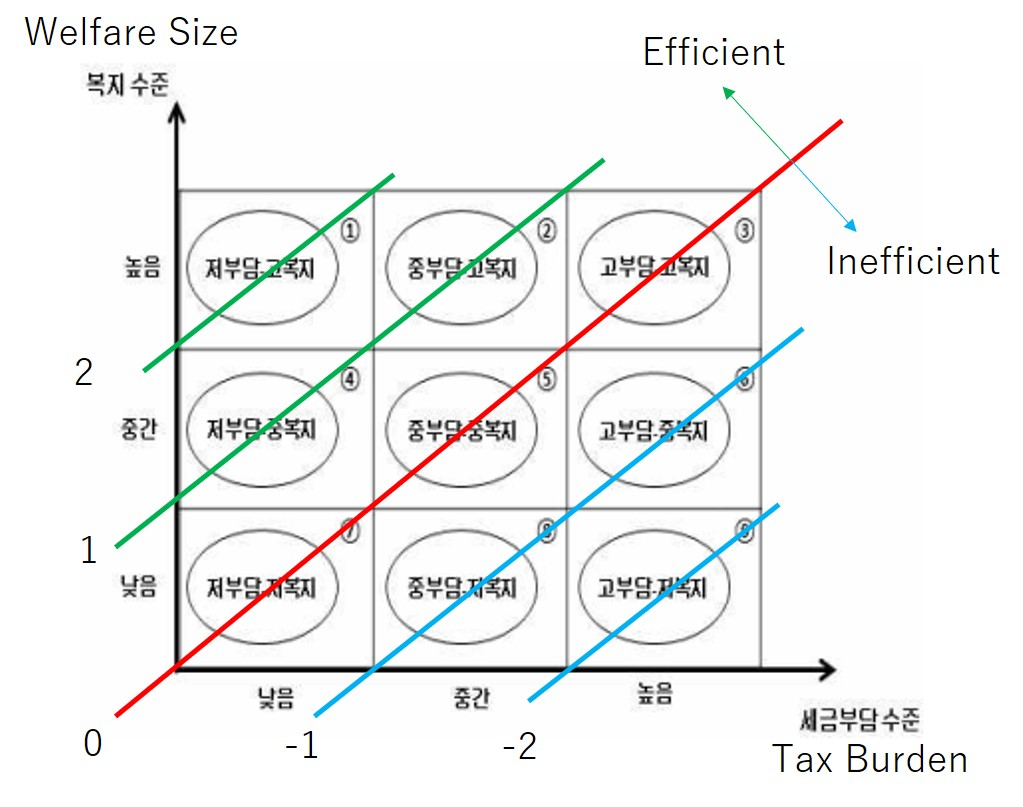
\includegraphics[width=0.5\textwidth,height=\textheight]{_assets/BalanceQuestion.jpg}
  
  To rule out government's policies, we use individual fixed effect as the \textbf{efficient index}
  
  \hypertarget{histrogram-of-efficient-index}{%
  \subsection{Histrogram of Efficient Index}\label{histrogram-of-efficient-index}}
  
  \begin{figure}
  
  {\centering 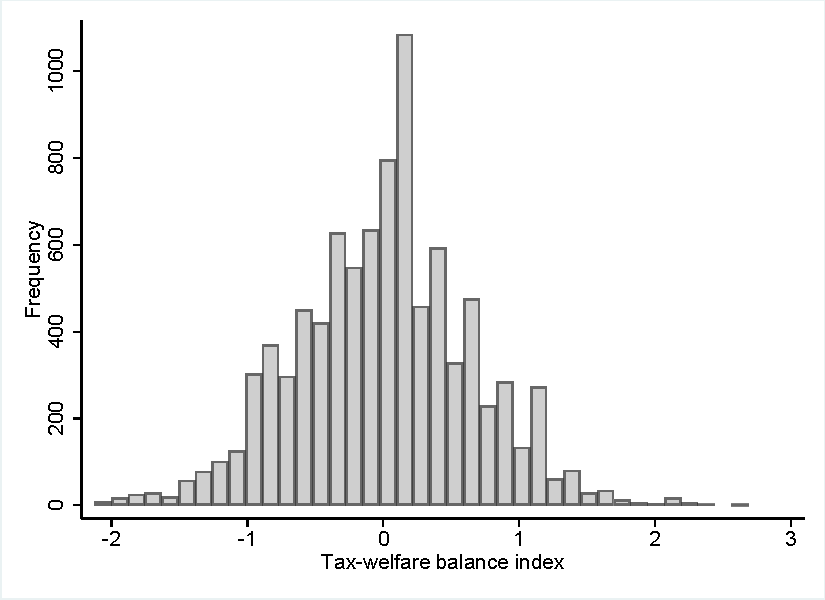
\includegraphics[width=0.9\linewidth]{C:/Users/vge00/Desktop/NaSTaB/_assets/HistogramBalanceid} 
  
  }
  
  \caption{Histogram of Efficient Index}\label{fig:unnamed-chunk-1}
  \end{figure}
  
  \hypertarget{heterogenous-price-elasticity-by-governement-efficiency}{%
  \subsection{Heterogenous Price Elasticity by Governement Efficiency}\label{heterogenous-price-elasticity-by-governement-efficiency}}
  
  To see the heterogenous price elasticity by efficient index,
  We estimated the baseline regression model (5) (see Table \ref{tab:kableEstimateElasticity}),
  using sample grouped by the efficient index.
  
  \begin{itemize}
  \tightlist
  \item
    Three quantile groups: we divide units \(i\) into the first, second, and third quantile of efficient index (1Q, 2Q, and 3Q, respectively).
  \end{itemize}
  
  \hypertarget{efficient-groups-estimation-results}{%
  \subsection{Efficient Groups: Estimation Results}\label{efficient-groups-estimation-results}}
  
  \hypertarget{robustness-check-2}{%
  \subsection{Robustness Check}\label{robustness-check-2}}
  
  \begin{enumerate}
  \def\labelenumi{\arabic{enumi}.}
  \tightlist
  \item
    Efficient index captures both government efficiency on concerns about budget deficits
  \item
    Effect of presidential transition on efficient index
  \item
    Effect of presidential transition on donation behavior
  \item
    Income and donations are determined simultaneously
  \item
    Last price elasticity
  \item
    Self-selection of receiving tax benefit
  \item
    Transitory and permanent elasticity
  \end{enumerate}
  
  \hypertarget{robustness-check-1-1}{%
  \subsection{Robustness Check 1}\label{robustness-check-1-1}}
  
  \begin{itemize}
  \tightlist
  \item
    Efficient index may capture both government efficiency on concerns about budget deficits
  
    \begin{itemize}
    \tightlist
    \item
      NASTAB asks respondents to answer the ideal balance b/w tax burdern and welfare size.
    \item
      We constructed the \textbf{ideal} efficient index, using the FE model to estimate the efficient index.
    \item
      We droped units with the ideal efficient index is less than 0 from each quantile group and repeated the same excercise.
    \item
      This is because respondents whose the ideal efficient index is less than 0 think governments should try to avoid budget deficits (high tax, low welfare).
    \end{itemize}
  \item
    Presidential transition effect on perceived efficiency
  
    \begin{itemize}
    \tightlist
    \item
      We constructed president-specific (ideal) efficient index and implemented the pair-wise t-test.
    \item
      As a result, average difference of these two indexs are not statistically siginificant zero.
    \end{itemize}
  \end{itemize}
  
  \hypertarget{robustness-check-1-estimation-results}{%
  \subsection{Robustness Check 1: Estimation Results}\label{robustness-check-1-estimation-results}}
  
  \hypertarget{robustness-check-2-1}{%
  \subsection{Robustness Check 2}\label{robustness-check-2-1}}
  
  We check the following two potential concerns
  
  \begin{itemize}
  \tightlist
  \item
    Presidential transition effect on donation behavior
  \item
    Income and donations are determined simultaneously
  \end{itemize}
  
  To address these problems, we estimated the FE model and Panel IV model with FE where instrument is \(\log(\text{Price}_{ijt}/\text{Price}_{ij(t-k)})\) for \(k = 1, 2, 3\), using data in 2013 and 2014.
  Moreover, we droped units with the ideal efficient index \textless{} 0 from each quantile group.
  
  Note that f-statistics of IV is greater than 500 when we estimate overall elasticity and extensive-margin elasticity, and greater than 100 when we estimate the intensive-margin elasticity.
  
  \hypertarget{robustness-check-2-result-1}{%
  \subsection{Robustness Check 2: Result}\label{robustness-check-2-result-1}}
  
  \hypertarget{robustness-check-2-result-extensive-margin}{%
  \subsection{Robustness Check 2: Result (Extensive Margin)}\label{robustness-check-2-result-extensive-margin}}
  
  \hypertarget{robustness-check-2-result-intensive-margin}{%
  \subsection{Robustness Check 2: Result (Intensive Margin)}\label{robustness-check-2-result-intensive-margin}}
  
  \hypertarget{conclusions}{%
  \section{Conclusions}\label{conclusions}}
  
  \hypertarget{conclusions-1}{%
  \subsection{Conclusions}\label{conclusions-1}}
  
  \clearpage
  
  \hypertarget{references}{%
  \subsection*{References}\label{references}}
  \addcontentsline{toc}{subsection}{References}

\end{document}


